\section{Lyttetest}
Da HRTF'er, som tidligere nævnt, ikke rigtigt kan generaliseres grundet menneskers meget individuelle udformninger af pinnaer, torsoer, hoveder osv., kan det være meget svært ud fra enkeltstående modultests at verificere hvor godt 3D-oplevelsen \textit{egentlig} funger.\\
Derfor udføres en kontrolleret lyttetest, for at få undersøgt om almindelige mennesker er i stand til at udpege en position af en lydkilde, ud fra den benyttede HRTF-database.  

\subsection{Forsøgsdeltagere}

For at indskrænke og sikre konkrete og fornuftige data, er det nødvendigt at fjerne så mange naturlige fejlkilder som muligt og udnytte testpersonernes evne til at lytte. 

Da projektet har til formål at udvikle generelt velfungerende 3D-lyd, er der ikke sat nogle særlige krav for testpersonernes køn eller alder. Ligeledes er det ikke anset for nødvendigt at teste deres hørelse, da de anses for at have to normalt-fungerende ører. \\
For at gøre det helt simpelt for deltagerne, gives alene informationen om, at de skal forsøge at sætte en position på lyden i forhold til deres eget hoved. Dermed bør der ikke komme stort udsving på folks forståelse af diverse testparametre. 

\subsection{Praktisk Setup}

I test-systemets natur med høretelefoner, udføres testen én af gangen, i fuld længde. Forsøgspersonen har selv mulighed for at skrue op eller ned for signalet efter behov, da hvert testsignal indeholder et reference-signal som lydniveauet kan holdes op imod for hver test. 

Testen udføres med det samme sæt høretelefoner for samtlige deltagere, for at gøre testen så ens som muligt for alle.

\subsection{Subjektive Parametre}
Under testen, skal forsøgspersonerne forsøge at klarlægge 3 parametre for hvert test-signal: Den horisontale position (Azimuth), den vertikale position (Elevation) og distance. 

Netop for at kunne forklare testparametrene til alle, benyttes 'horisontal' og 'vertikal', istedet for Azimuth og Elevation, da disse begreber er mere alment kendt, og tilstrækkende dækkende betegnelser under test. 

\subsection{Præsentationsmetode}

Testen består af 10 testsignaler, som alle er opsat efter en AB-testsekvens, som illustreret på figur \ref{fig:ABTest}. 

\figur{1}{ABTest}{AB Testsekvens \cite{Lyttetest}}{ABTest}

I hvert testsignal udgør A et referencepunkt i $0\deg$ Azimuth, $0\deg$ Elevation og 1 meters afstand, hvor B vil være positionen under test. 
Hvert testsignal er af 10 sekunders varighed, og afspiller et talesignal, overlejret med musik. 

For at give forsøgspersonerne ekstra godt grundlag at evaluere positionen på, gentages AB sekvensen to gange i træk (ABAB), for derefter at give 10 sekunders evalueringstid.
Dette giver hvert teststykke en varighed af 50 sekunder, med en samlet testtid på lige omkring 8½ minut pr forsøgsperson. 
Dette giver en samlet testtid, såfremt der ikke ønskes gentagelser af en test, på omtrent 1½ time.

%Valget af positioneringernes rækkefølge er valgt tilfældigt, men er dog valgt med henblik på at teste både de nemme positioner (lige ud for et øre), samt de psykoakustisk sværere scenarier for for/bag-forvirring og lige over hovedet.

\subsection{Bedømmelsesskala}

Da testen kun bekymrer sig om forsøgspersonernes evne til at kunne lokalisere positionen for en given lydkilde, er der forsøgt at gøre bedømmelsen så simpel som muligt. \\
Ved at give 3 parametre som blot skal afmærkes på 3 figurer, som det ses på figur \ref{fig:lyttetesteksempel}, kan forsøgspersonerne forholde sig meget naturligt til bestemmelse af lydkildens position.

\figur{1}{lyttetesteksempel}{Eksempel for bedømmelse af position}{lyttetesteksempel}

Denne intuitive bedømmelsesskala kræver netop heller ikke at forsøgspersonerne nødvendigvis tænker i konkrete tal og vinkler, men giver deres istedet mulighed for deres umiddelbare, subjektive oplevelse af lydens position. 

\subsection{Opsummering}

For hurtigt at grænse lyttetesten op, listes her valgene for testen:

\begin{itemize}
	\item 10 Forsøgspersoner - Ingen krav til køn eller alder
	\item Forsøgspersoner får at vide at de skal bedømme lydens position
	\item Test med høretelefoner - én af gangen
	\item Valgfrit lydniveau
	\item Testsignaler må gentages
	\item Der testes for Azimuth, Eleation og Distance for hvert signal
	\item Signalerne præsenteres med AB-sekvens
	\item Sekvens gentages to gange pr testsignal.
	\item Testlængde for én person: 8½ Minut
	\item Testlængde samlet: 1½ Time
	\item Bedømmes efter markering på illustration
	
\end{itemize}
%på 9 antal vilkårlige testpersoner. Lyttetesten går ud på at de ud fra 10 specifikke testsignaler skal bedømme hvor de mener at lydkilden er placeret og notere både azimuth, elevation og distance. De 10 testsignaler er en blanding af speak og musik, hvor rækkefølgen er ABABA hvor A henviser til referencepunktet [1,0,0], og B henviser til den position som skal bestemmes af testpersonen. Hvert signal afspille i 10 sekunder.
%Testen er udført med musikken afspillet fra en mobiltelefon (hhv en Huawei P10 Lite og en One Plus 2), og høretelefonerne er JBL Everest 300. Testpersonerne kunne afspille hvert testsignal så mange gange de ønskede. Signalerne er designet til at teste virkningsgraden af azimuth, elevation og distance, både hver for sig og i kombinationer. Derudover testes der på nogle psykoakustiske 'svære' placeringer, som f.eks. $180\deg$ azimuth eller $90\deg$ elevation.  
%\fxnote{Obs på volumen og hvilken info de skal have LS}

%\begin{figure}[h!]
%	\centering
%	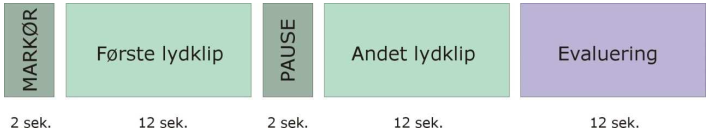
\includegraphics[width=0.7\linewidth]{All_Pics/ABtest}
%	\caption{}
%	\label{fig:abtest}
%\end{figure}
